\hiddenappendixchapter
    {Application Launch and Interface Overview}
    {app:application_interface_overview}

\section{Inspection and Conductor Modules}
\label{appsec:inspection_modules}

The model-inspection and conductor-analysis tabs follow the general interface
organisation described in Chapter~6. The following views show each area
separately so that its main selectors, controls and output regions can be
identified clearly.

\begin{figure}[p]
    \centering
    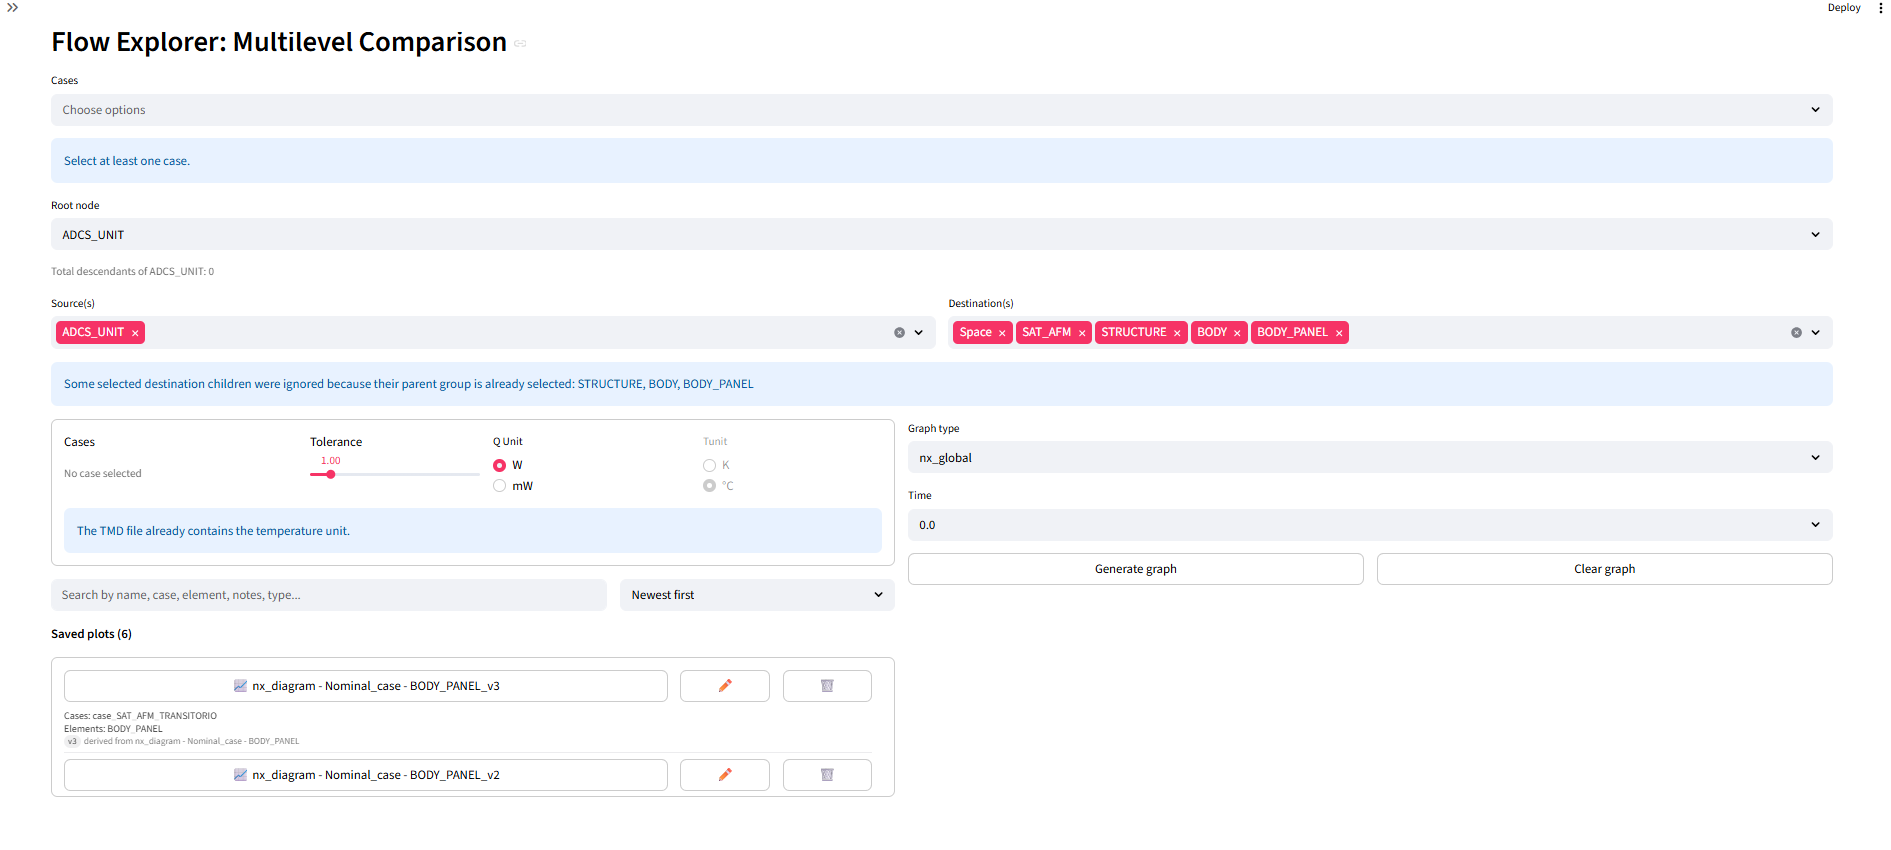
\includegraphics[
        width=\textwidth,
        height=0.76\textheight,
        keepaspectratio
    ]{Figures/Anexo_01/display01.png}
    \caption{Flow Explorer interface for hierarchical heat-flow inspection
    and multi-case representation.}
    \label{fig:appendix_flow_explorer}
\end{figure}

\clearpage

\begin{figure}[p]
    \centering
    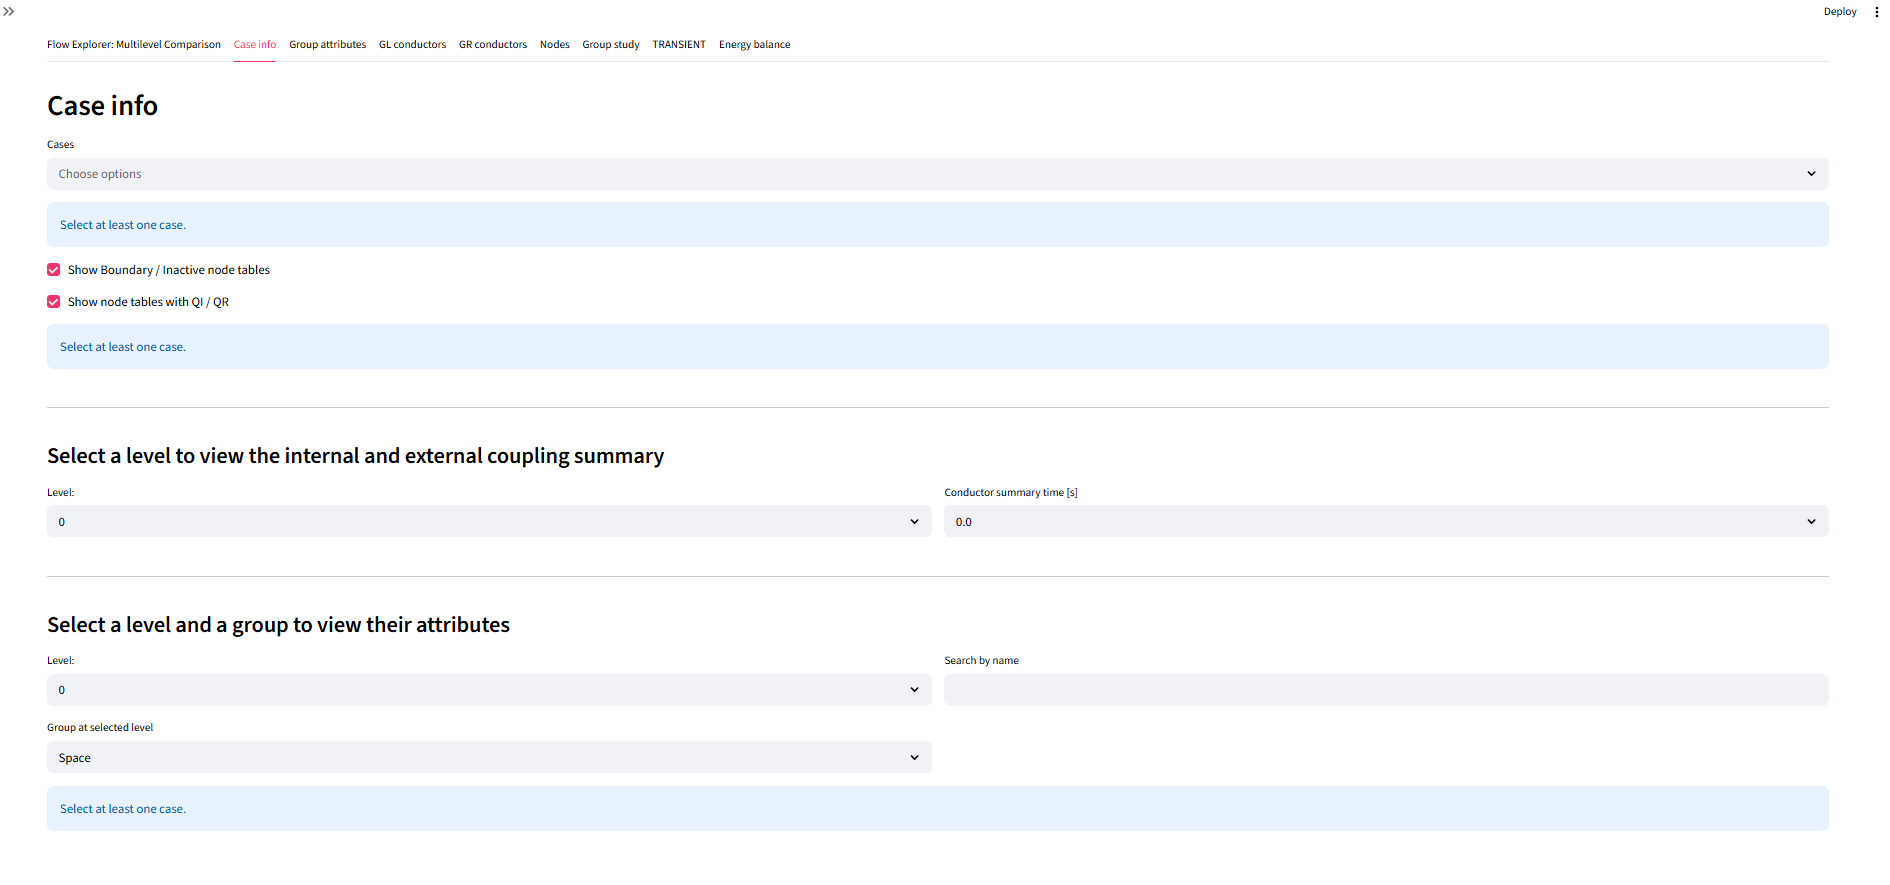
\includegraphics[
        width=\textwidth,
        height=0.76\textheight,
        keepaspectratio
    ]{Figures/Anexo_01/display02.png}
    \caption{Case-information interface showing the datasets, groups and
    couplings available in the loaded simulation.}
    \label{fig:appendix_case_information}
\end{figure}

\clearpage

\begin{figure}[p]
    \centering
    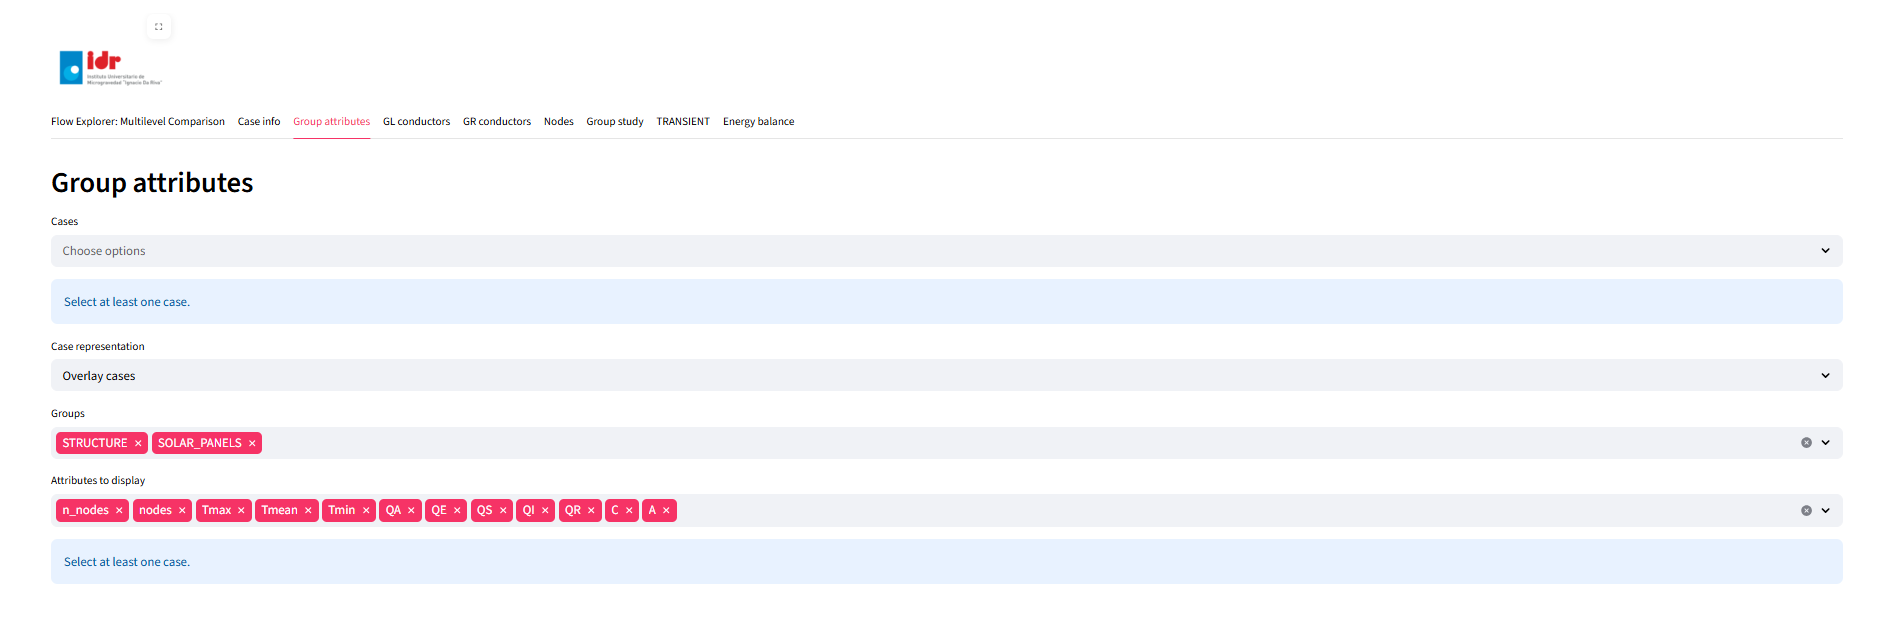
\includegraphics[
        width=\textwidth,
        height=0.76\textheight,
        keepaspectratio
    ]{Figures/Anexo_01/display03.png}
    \caption{Group-attribute interface for inspecting the selected model
    elements at a specified output instant.}
    \label{fig:appendix_group_attributes}
\end{figure}

\clearpage

\begin{figure}[p]
    \centering
    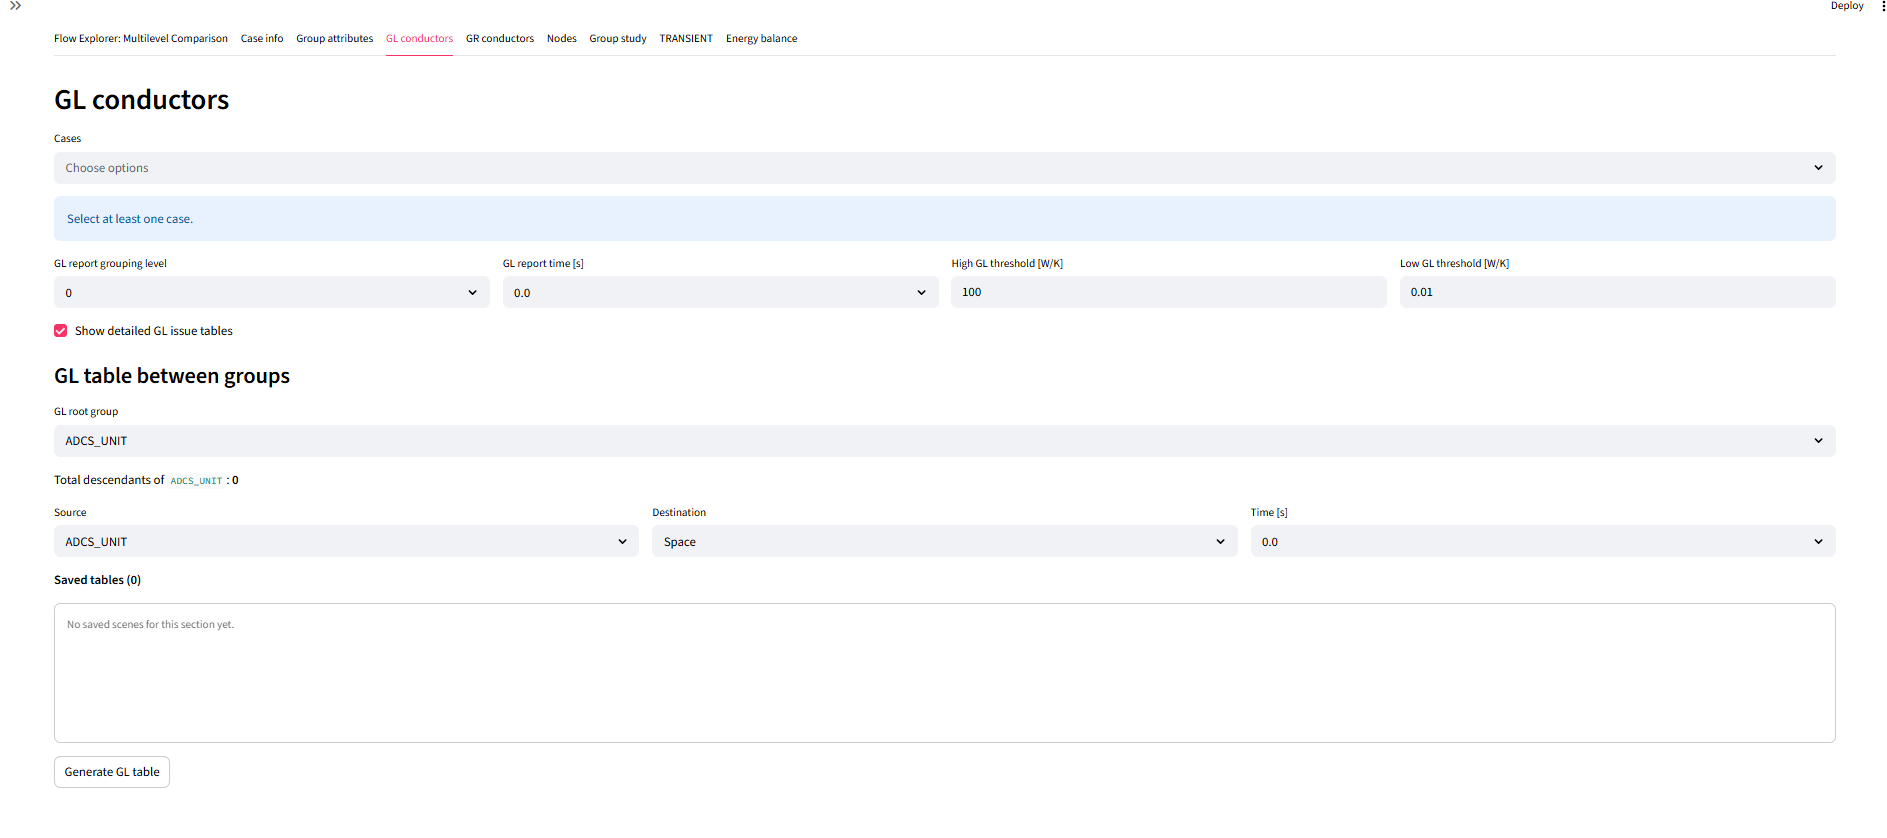
\includegraphics[
        width=\textwidth,
        height=0.76\textheight,
        keepaspectratio
    ]{Figures/Anexo_01/display04.png}
    \caption{Linear-conductor interface with case, group and output-time
    controls.}
    \label{fig:appendix_gl_conductors}
\end{figure}

\clearpage

\begin{figure}[p]
    \centering
    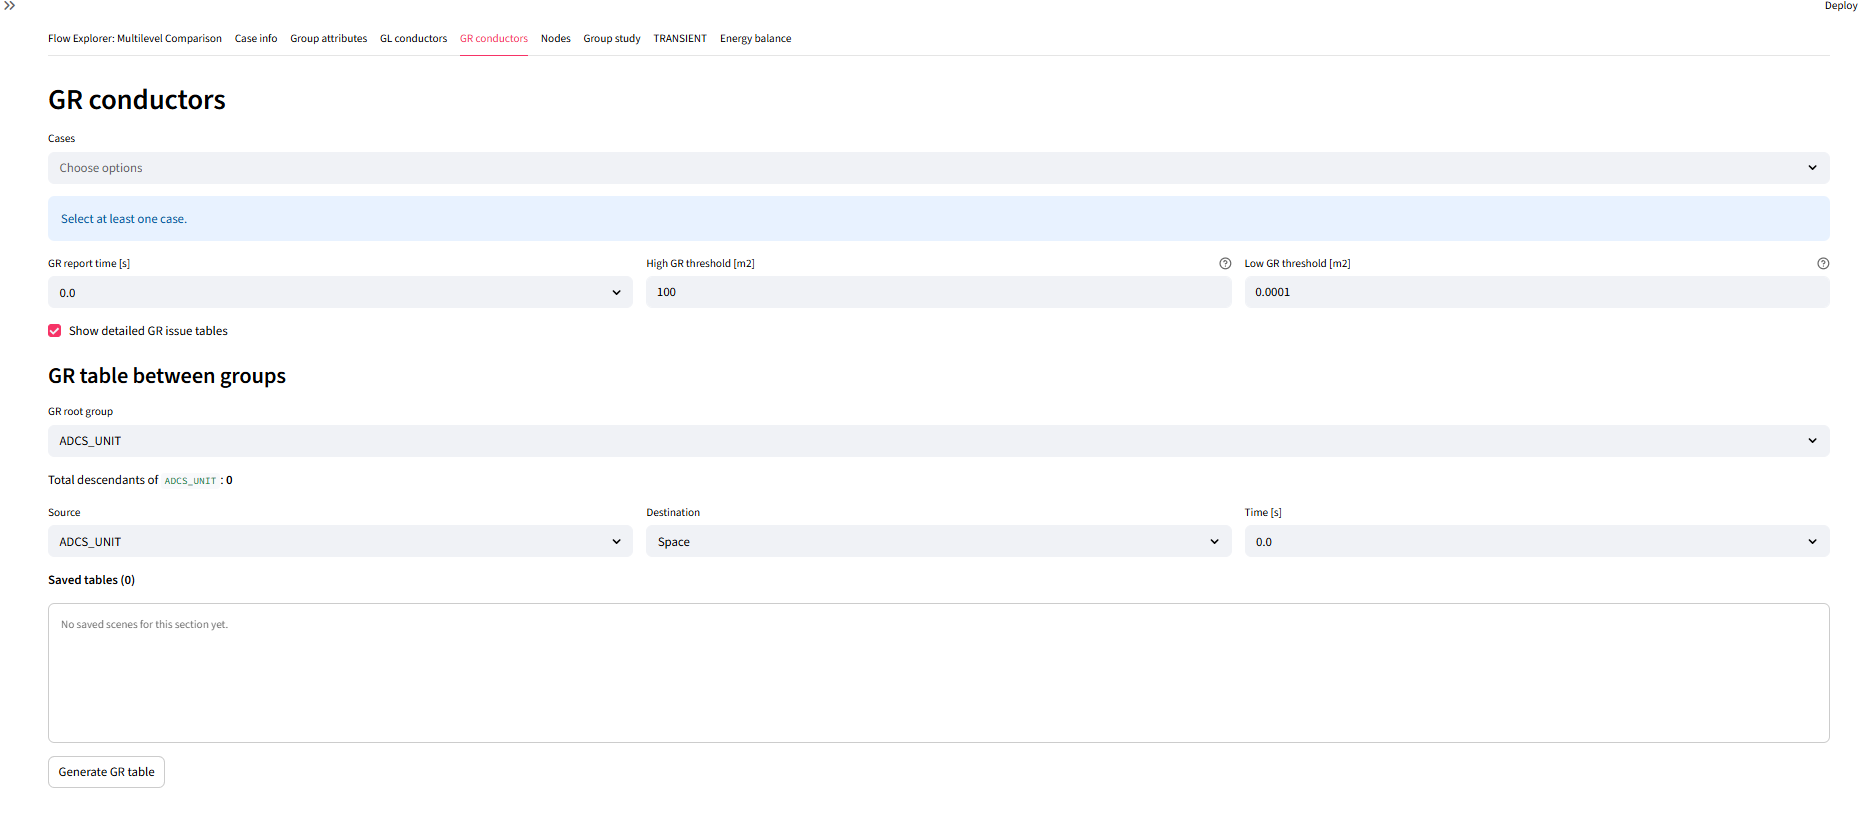
\includegraphics[
        width=\textwidth,
        height=0.76\textheight,
        keepaspectratio
    ]{Figures/Anexo_01/display05.png}
    \caption{Radiative-conductor interface with case, group and output-time
    controls.}
    \label{fig:appendix_gr_conductors}
\end{figure}

\clearpage

\begin{figure}[p]
    \centering
    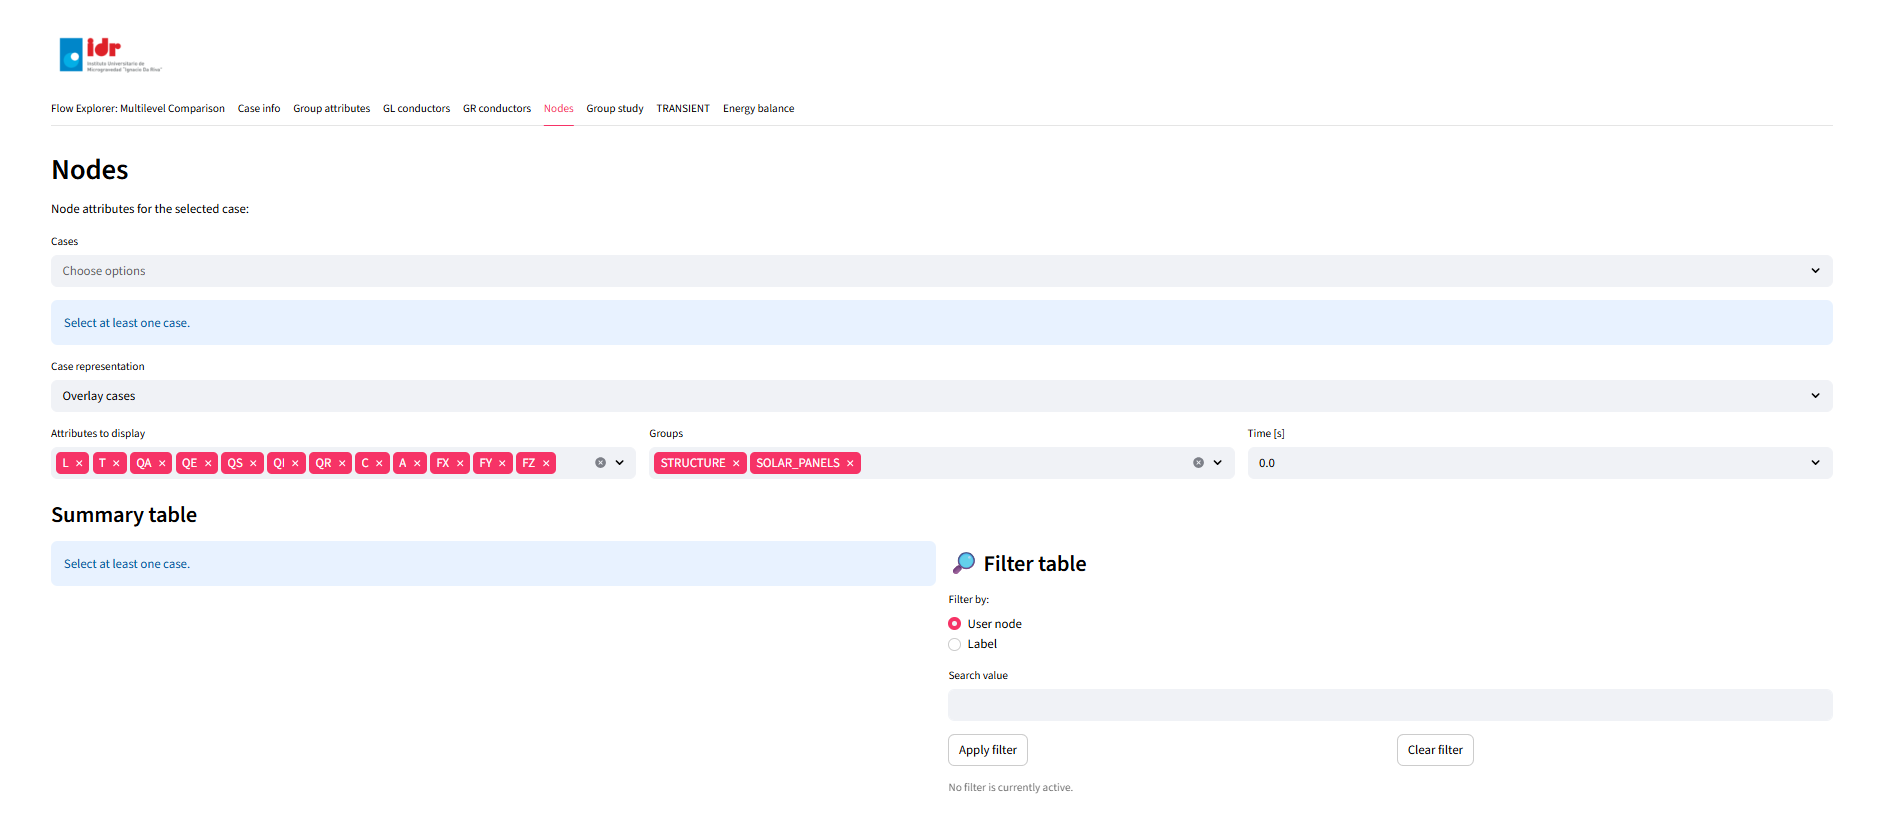
\includegraphics[
        width=\textwidth,
        height=0.76\textheight,
        keepaspectratio
    ]{Figures/Anexo_01/display06.png}
    \caption{Nodal-information interface for the selected hierarchy
    elements.}
    \label{fig:appendix_nodes}
\end{figure}

\clearpage

\begin{figure}[p]
    \centering
    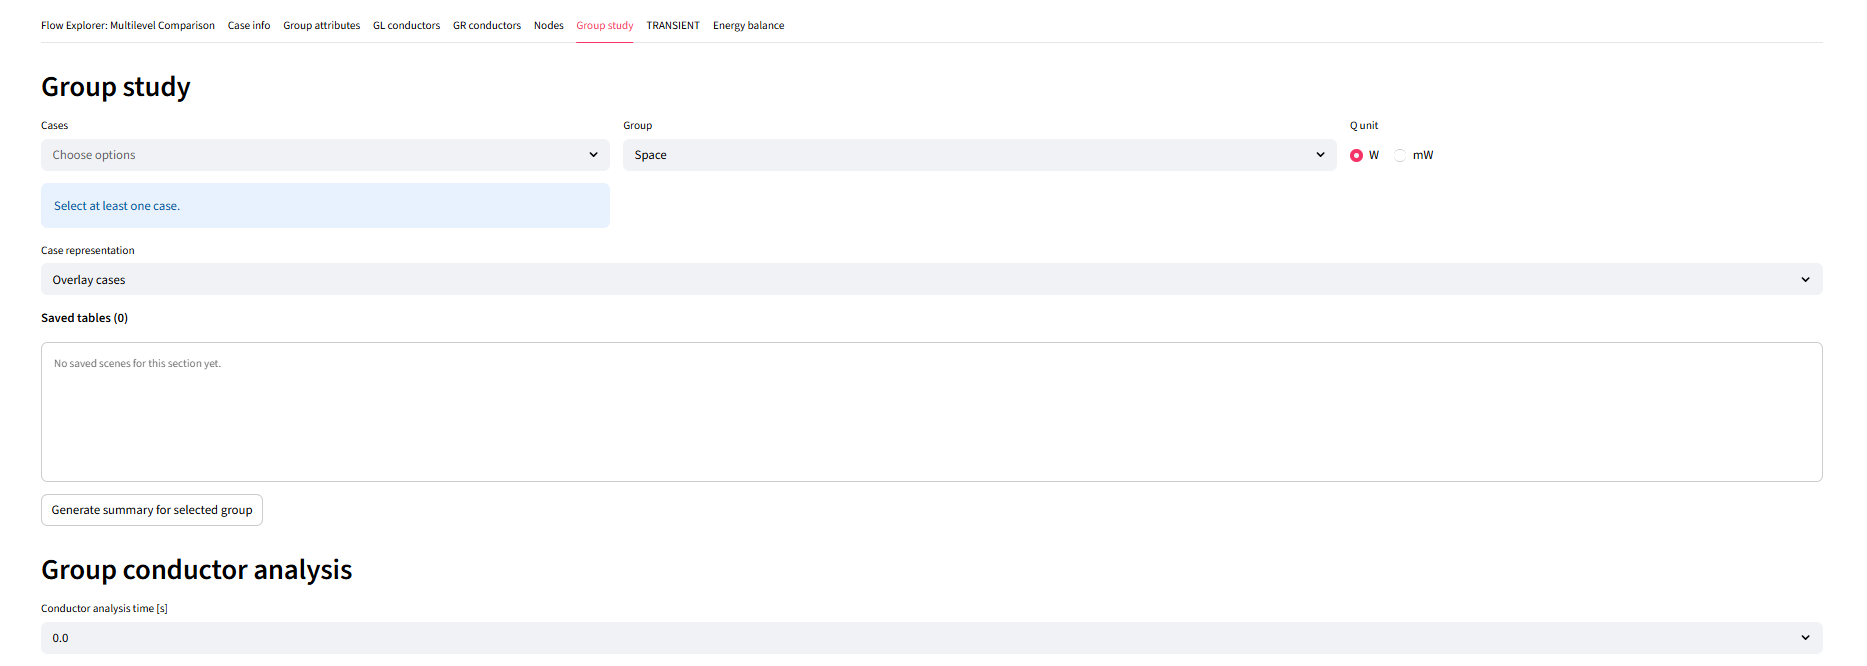
\includegraphics[
        width=\textwidth,
        height=0.76\textheight,
        keepaspectratio
    ]{Figures/Anexo_01/display07.png}
    \caption{Group-study interface for the inspection of selected components
    and their thermal connections.}
    \label{fig:appendix_group_study}
\end{figure}

\clearpage